\documentclass[a4paper,11pt]{article}
\usepackage{lecturenotes}
\lectureheader{ELE745}{4}
\begin{document}
\tableofcontents
\clearpage
\noteheading{1}{Random Variable and Random Processes - Review}
\notedefinition{Probability Definition}{
    Probability is defined on events. For an event $A \subseteq S$ occurring $n(A)$ times in $n$ trials of a random experiment with sample space $S$, its probability is
    \[
        P(A) = \lim_{n \to \infty} \frac{n(A)}{n}.
    \]
    
    \tcblower

    \textbf{Axioms of Probability}
    \begin{itemize}
        \item Probability is a non-negative number - $P(A) \geq 0$
        \item Probability of the whole set is unity - $P(S) = 1$
        \item For any countable collection $A_{1},A_{2},\dots$ of mutually exclusive events,
        \[
            P(A_{1} \cup A_{2} \cup \dots) = P(A_{1}) + P(A_{2}) + \dots
        \]
    \end{itemize}
}

\notedefinition{Conditional Probability}{
    Conditional probability is defined as:
    $$
    P(A|B) = \frac{P(AB)}{P(B)} \ P(B) \neq 0
    $$
}

\noteheading{2}{Independent Events}
Two events A and B are said to be independent if: $P(AB) = P(A)P(B)$. If A and B are independent then:
$$
P(A|B) = P(A)
$$

\textit{A provides no insight into the event of B, and vice-versa}

\noteheading{2}{Laws of Total Probability}
Conditional probability can express the probability of a complicated event in terms of simpler events. If $A_{1}, A_{2}, \dots, A_{n}$ are \textit{pair-wise disjoint} and their union is, then: $A_{i} \cap p A_{j} = \phi \ \text{(null-set)}$, and
$$
U_{i=1}^{n} A_{i} = S
$$

By expanding: $B = BS$ and $A_{i} \cap A_{j} = \null \implies BA_{i} \cap BA_{j} = \phi$

\keyequation{Law of Total Probability}{P(B) = \sum^n_{i=1}P(BA_{i}) = \sum_{i=1}^n P(B|A_{i})P(A_{i})}

\Needspace{9\baselineskip}
\begingroup
\definecolor{NoteAccent}{HTML}{477A35}
\notebox{Example: Defective Bulbs}{
    $B_1$: 100 bulbs, 15 defective;\quad $B_2$: 200 bulbs, 5 defective.

    Choose either box with probability $1/2$, then a random bulb. Let $D$ denote a defective bulb.
    \setlength{\abovedisplayskip}{5pt}
    \setlength{\belowdisplayskip}{0pt}
    \[
        P(D) = \sum_{i=1}^{2} P(D\mid B_i)P(B_i)
        = \frac{1}{2}\left(\frac{15}{100} + \frac{5}{200}\right)
        = 0.0875 = \boxed{8.75\%}.
    \]
}
\endgroup

A more general version of Bayes theorem involves a partition of S:
\keyequation{General Form of Bayes Theorem}{P(B|A_{i}) = \frac{P(B|A_{i})P(A_{i})}{\sum_{j=1}^n P(B|A_{j})P(A_{j})}}[
    In the above equation, $A_{i}, i = [1,n]$ represent a set of mutually exclusive events with associated 'a priori' probabilties $P(A_{i}), i = [1,n]$. Meaning that with the information that B has occured, 
    the information about $A_{i}$ can be updated by the n conditional probabilities: $P(B|A_{j}), j = [1,n]$
]

\noteheading{1}{Random Variables, PDFs, and CDFs}
\noteheading{2}{Important Definitions and Distributions}

\textbf{Random Variable (X,Y,Z, $\dots$):} A rule for assigning a real number to every outcome of an experiment \\
\textbf{Cumulative Distribution Function (CDF):} $F_{X}(x) = P(X \leq x$) \\
\textbf{Probability Mass Function (PMF):} \textit{For discrete random variables} 
$$
\begin{aligned}
    P_{X}(X_{i}) &= P(X=X_{i}) \\
    P(a\leq x \leq b) &= \sum_{X_{i} \in [a,b]} P(X=X_{i}) \\
    \sum_{X_{i}} P(X=X_{i}) &= 1
\end{aligned}
$$
\textbf{Probability Density Function (PDF)}: \textit{For continuous random variables}
$$
\begin{aligned}
    f_{X}(x) &= \frac{dF_{X}(x)}{dx} \\
    P(a \leq  X \leq  b) &= \int^b_{a} f_{X}(t) dt \\
    \int^\infty_{-\infty} f_{X} (t) dt &= 1
\end{aligned}
$$
\keyequation{Uniform Distribution in $[a,b]$}{
    f_{X} (x) = \begin{cases}
        \frac{1}{b-a} & (a \leq x \leq b) \\
        0 & \text{otherwise}
    \end{cases}
}
\keyequation{Gaussian (normal) Distribution ~ $N(\mu,\sigma^2)$}{
    f_{X}(x) = \frac{1}{\sqrt{2\pi}\sigma} \exp (-\frac{(x-\mu)^2}{2\sigma^2}) \quad -\infty<x<\infty
}
If X and Y are independent: $f_{XY}(x,y) = f_{X}(x) f_{Y}(y)$

\noteheading{2}{Gaussian Random Variables}
If $f_{X}(x)$ is a gaussian distribution, it is a bell-shaped curve symmetric around the parameter: $\mu$
\begin{notation}
$\mu$ & unit variance & N/A \\
$\sigma$ & mean & N/A \\
\end{notation}

\notedefinition{Normalized Gaussian RV Y}{Let Y follow a Gaussian distribution with zero mean and unit variance:
$$
f_{Y}(y) = \frac{1}{\sqrt{2\pi}}\exp [-\frac{x^{2}}{2}]
$$

Denoted as $Y ~ N(0,1)$

\tcblower
\textbf{Distribution Function of Y:} 
$$
P(Y\leq y) = F_{Y}(y) = \int_{-\infty}^y \frac{1}{\sqrt{2\pi}} \exp [-\frac{m^{2}}{2}] dm = 1 - Q(y)
$$

Where Q(y) is the \textbf{Standard Normal Complementary CDF (tail probability)} and is defined as:
$$
Q(y) = P(Y\geq y) = \int_{y}^{\infty} \frac{1}{\sqrt{2\pi }\exp [-\frac{m^{2}}{2}]dm}
$$

\tcblower
\textbf{Properties of Q-Function}
\begin{itemize}
    \item $Q(-y) = 1 - Q(y)$
    \item $P(a\leq Y\leq b) = Q(a) - Q(b)$
\end{itemize}
}

\Needspace{23\baselineskip}
\notedefinition{Tail Probability of a General Gaussian RV}{
For $X \sim N(\mu,\sigma^2)$ with mean $\mu$ and variance $\sigma^2$,
\[
\begin{aligned}
    P(X>x)
    &= \int_x^\infty \frac{1}{\sigma\sqrt{2\pi}}
       \exp\!\left(-\frac{(\tau-\mu)^2}{2\sigma^2}\right)\,d\tau \\
    &\overset{t=\tau-\mu}{=}
       \int_{x-\mu}^\infty \frac{1}{\sigma\sqrt{2\pi}}
       \exp\!\left(-\frac{t^2}{2\sigma^2}\right)\,dt \\
    &= \int_{x-\mu}^\infty \frac{1}{\sqrt{2\pi}}
       \exp\!\left(-\frac{(t/\sigma)^2}{2}\right)\,\frac{dt}{\sigma} \\
    &\overset{u=t/\sigma}{=}
       \int_{(x-\mu)/\sigma}^\infty \frac{1}{\sqrt{2\pi}}
       \exp\!\left(-\frac{u^2}{2}\right)\,du.
\end{aligned}
\]
\keyequation{Gaussian Tail Probability}{
    P(X>x) = Q\!\left(\frac{x-\mu}{\sigma}\right)
}

\tcblower

The probability of the Gaussian RV: $X ~ N(\mu, \sigma^2)$, can be determined using the previous property of the normalized Gaussian RV: $Y = \frac{X-\mu}{\sigma} ~ N(0,1)$. Then the probability of X can be solved using a Q-function:
\keyequation{RV X ~ $N\mu, \sigma^2$ in terms of the Q-function}{P(a\leq X\leq b) = Q(\frac{a-\mu}{\sigma}) - Q(\frac{b-\mu}{\sigma})}
}

\noteheading{1}{Statistics}
\keyequation{Expectation (mean)}{\mu x = E[X] = \int_{-\infty}^{\infty} x f_{X}(x)dx}[
    The mean of U[a,b] is: \textbf{\textcolor{blue}{${b-a}/{2}$}} and the mean of $N(\mu,\sigma^2)$ is \textbf{\textcolor{blue}{$\mu$}}
]

\keyequation{Variance}{\sigma^2_{X}=E[(X-\mu x)^2] = E(X^{2}) - \mu^2_{X} = \int_{-\infty}^{\infty} x^{2} f_{X}(x)dx - \mu^2_{X}}[
    The variance of U[a,b] is \textbf{\textcolor{blue}{$(b-a)^2/12$}} and the variance of $N(\mu ,\sigma^2)$ is \textbf{\textcolor{blue}{$\sigma^2$}}
]

\noteheading{1}{Power and Power Spectral Density (PSD)}
Recall the average power of a deterministic signal, with Parsevals Theorem, we can express it in both time and the frequency domain.
\keyequation{Parsevals Theorem}{P = \int_{-\infty}^{\infty} \lim_{T \to \infty} \frac{1}{T} |X_{T}(f)|^{2} df = \int_{-\infty}^{\infty} S_{X}(f)df}[
    Where $S_{X}(f) = \lim_{T \to \infty} \frac{1}{T}|X_{T}(f)|^{2}$ is the \textbf{PSD} of x(t)
]
\noteheading{2}{PSD of a Random Signal}
For a random signal X(T):
$$
P = \int_{-\infty}^{\infty} S_{X}(f)df
$$

\textbf{Properties:}
\begin{itemize}
    \item $S_{X}(f) \geq 0$ for any f
    \item $S_{X}(f) = S_{X}(-f)$
    \item $S_{Y}(f) = |H(f)|^{2} \cdot S_{X}(f)$
\end{itemize}

The third property only applies to WSS (wide-sense stationary processes).

\notedefinition{White Gaussian Noise}{
    The random process N(t) is called \textbf{white gaussian noise} if N(t) is a Gaussian RV at any time instant t with:
    $$
    E[N(t) N(t-\tau )] = \frac{N_{0}}{2}\delta(\tau)
    $$
    and $E[N(t)] = 0$, $\frac{N_{0}}{2}$ is called a two-sided PSD.
    \tcblower
    \textbf{Properties}
    \begin{itemize}
        \item $E[N(t_{1})N(t_{2})] = 0$ if $t_{1} \neq t_{2}$
        \item $E[N^{2}(t)] = \infty$ N(t) is physically unrealizable
        \item $S_{N}(f) = \frac{N_{0}}{2}$ for $-\infty < f < \infty$ (Two-sided PSD)
    \end{itemize}
}

\par\addvspace{7pt}
\noindent\begin{minipage}{\linewidth}
    \centering
    \captionsetup{hypcap=false,type=figure}
    \includegraphics[width=0.6\linewidth,keepaspectratio]{figures/AWGN-noise.png}
    \caption{White Gaussian Noise Example}
    \label{fig:}
\end{minipage}
\par\addvspace{7pt}

\noteheading{1}{White Gaussian Noise Passing a LTI System}
Let N(t) be a White Gaussian noise passing an LTI system with impulse response h(t) and the transfer function of H(f).
\par\addvspace{7pt}
\noindent\begin{minipage}{\linewidth}
    \centering
    \captionsetup{hypcap=false,type=figure}
    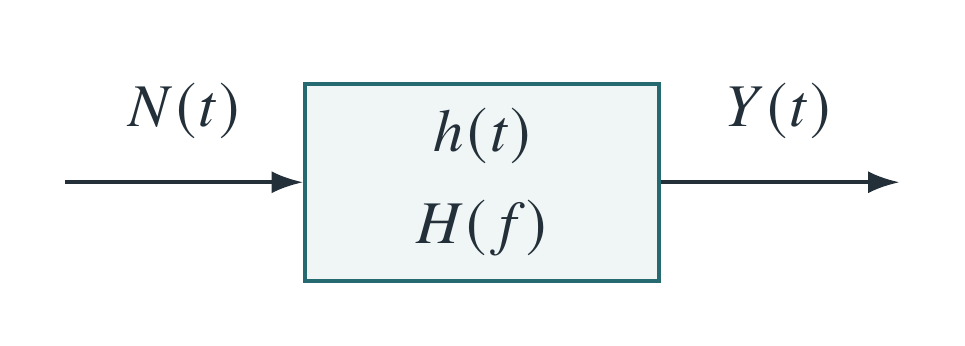
\includegraphics[width=0.6\linewidth,keepaspectratio]{figures/noise-filter-block-diagram.png}
    \caption{White Gaussian w.r.t LTI System}
    \label{fig:}
\end{minipage}
\par\addvspace{7pt}
\keyequation{Output of Above LTI System}{S_{Y}(f) = |H(f)|^{2}S_{N}(f) = \frac{N_{0}}{2}|H(f)|^{2}}
\vspace{6pt}
\keyequation{Average Power of Above LTI System}{E[Y^{2}(t)]=\int_{-\infty}^{\infty}S_{Y}(f) df = N_{0}/2 \int_{-\infty}^{\infty} |H(f)|^2 df = \sigma_Y^2}








\end{document}
